\chapter{Automated Sparse Tiling for Irregular Computations}
\label{ch:sparsetiling}

\section{Motivation}
\label{sec:tiling:motivation}
%mention dichotomy tiling/fusion...

%- irregular codes from pde-land are often memory bound (this however depends on the discretization)
%- investigation of tiling in real-world irregular codes

%- fully parallel loops ! with local reductions ... (diff with global reductions)



Many numerical methods for partial differential equations (PDEs) are structured as sequences of parallel loops. This exposes parallelism well, but does not convert data reuse between loops into data locality, since large datasets are usually accessed. In Section~\ref{sec:bkg:poly} we have explained that loop fusion and loop tiling may be used to retain some of this potential data locality. As we elaborate in the upcoming sections, however, it is extremely challenging to implement these optimizations in most real-world applications. 

Our focus is on unstructured mesh PDE solvers, like those based on the finite volume or the finite element methods. Here, the  loop-to-loop dependence structure is data-dependent due to
indirect references such as \texttt{A[map[i]]}; the \texttt{map} array stores connectivity information, for example from elements in the mesh to degrees of freedom. A similar pattern occurs in molecular dynamics simulations and graph processing, so both the theory and the tools that we will develop in this chapter are generalizable to these domains. 

Because of the irregular memory access pattern, our approach to loop transformation is based on dynamic analysis, particularly on \textit{inspector/executor schemes}. Our hypothesis, backed by the studies reviewed in Section~\ref{sec:bkg:ie}, is that dynamic loop optimization can improve the performance of a class of real-world unstructured mesh applications. Among the possible dynamic loop optimizations, we target \textit{sparse tiling}. We recall from Section~\ref{sec:bkg:tiling} that sparse tiling aims to exploit data reuse across consecutive loops by composing two transformations, namely loop fusion and loop tiling. 

Summarizing, the three main issues that we tackle in this chapter are:

\begin{itemize}
\item Previous approaches to sparse tiling were all based upon ``ad-hoc'' inspector/executor strategies; that is, developed ``by hand'', per application. We seek for a general technique, applicable to arbitrary computations on unstructured meshes.
\item Automation is more than a desired feature because application specialists avoid complicated optimizations that can harm the comprehensibility of source code. We therefore aim for a fully-automated framework, based upon a mixed compiler/library approach.
\item Very few studies have tackled the problem of fusing loops when these are interleaved by routines for message passing. We are aware of none for the case in which the memory accesses pattern is irregular, as in unstructured mesh applications. We fill this gap employing a mixed split/overlapped sparse tiling scheme. This is a fundamental contribution since most scientific simulations run on distributed-memory architectures.
\end{itemize}

\section{Open Problems, Questions, Hypotheses}
\label{sec:tiling:struct}
Loop fusion and loop tiling have widely been studied in the literature. Over the years, a significant number of compilers and techniques have been proposed for automating these transformations. Their evaluation, however, has mostly been limited to a small set of benchmarks (or ``mini-applications'') and single-node performance. This unfortunately does not shed light on the applicability in real-world applications, where the loop nests are often deeper, less structured, and characterized by irregular control flow. On the other hand, it is true that simple stencil codes arising in finite difference methods~\citep{vect-tiled-ho-fd,ics-stencil-tiling,cohen-timetiling}, linear algebra routines~\citep{qr-fact-tiled,blas-tiling}, and image processing kernels~\citep{Halide} can really benefit from transformations like fusion and tiling. Since numerical methods for partial differential equations (PDEs) are often structured as sequences of parallelizable loops (or ``sweeps'') over the discretized equation domain, the following questions arise naturally: 

\begin{description}
\item[Applicability] Can we adopt sparse tiling in real-life numerical methods for solving PDEs, and should we expect any gain in performance?
\item[Lack of evidence] Why, despite decades of research, loop transformations are rarely used in production code? 
\item[Challenges] What are the theoretical and technical challenges that we have to overcome to automate sparse tiling?
\end{description}

The context in which we tackle these questions is the following:
\begin{description}
\item[Irregular codes] Unstructured meshes are often used to discretize the computational domain, since they allow for an accurate representation of complex geometries. Their connectivity is stored by means of adjacency lists (or equivalent data structure). This leads to indirect memory accesses within loop nests. Indirections break static analysis, thus making compiler-based approaches to loop transformation (e.g., polyhedral optimization) unsuitable for our context. Runtime data dependence analysis enables dynamic loop optimization, although at the price of additional overhead.
\item[Realistic datasets] Complex simulations usually operate on at least gigabytes of data, thus requiring multi-node execution. Any loop transformation we consider will have to support\ distributed-memory parallelism.
\item[Automation, but no legacy code] Sparse tiling is an ``extreme optimization''. It requires a great deal of effort to be implemented because it imposes a serious restructuring of the application. Similarly to many other low level transformations, it also tends to render the source code impenetrable, increasing the maintenance and the extension costs. We therefore aim for a fully automated system based on domain-specific languages, which abstracts sparse tiling through a simple interface (i.e., a simple construct that lets the users tell the compiler ``apply sparse tiling to the following sequence of loops'' ) and a tiny set of parameters for performance tuning (e.g., the tile size). We are not interested in supporting legacy code, where the key computational aspects (e.g., mesh iteration, distributed-memory parallelism) are usually hidden for software modularity, thus making automation almost impossible.
\end{description}

Based upon these observations and requirements, we decompose our problem into two tasks:
\begin{enumerate}
\item writing a library for expressing inspector/executor schemes (\cite{ST-Saltz91}) that enable sparse tiling in arbitrary computations on unstructured meshes;
\item integrating the library with a multilayer framework based on domain-specific languages.
\end{enumerate}
Before addressing these two tasks, respectively in Sections~\ref{sec:tiling:lc}-\ref{sec:tiling:algo} and Section~\ref{sec:tiling:automation}, we elaborate on the theoretical and technical challenges that arise when applying loop fusion and loop tiling to real codes (Section~\ref{sec:tiling:difficult}), and review the related work (Section~\ref{sec:tiling:relatedwork}).  

%Finally, to summarize, our hypotheses are:
%\begin{itemize}
%\item Many loop nests in unstructured mesh applications are memory-bound, so exploiting the data reuse across consecutive loop nests should improve the performance.
%\item Applying sparse tiling is extremely complicated, so automation is necessary. However, automation presents challenges that none of the existing technologies can overcome. \end{itemize}

% Is skewing used for optimizing cross-time dependency, i.e., is the wave due to time?

\section{Applying Fusion and Tiling is More Difficult than Commonly Thought}
\label{sec:tiling:difficult}
We show in Listing~\ref{code:tiling-struct} the ``skeleton'' of a typical PDE solver on an unstructured mesh. This will be useful throughout the analysis presented in this section.

\begin{algorithm}[t]
\scriptsize\ttfamily
\SetAlgorithmName{LISTING}{}

// Time-stepping loop (T = total number of iterations)\\
\KwSty{for} t = 1 \KwSty{to} T $\lbrace$\\
~~// 1st sweep over the $C$ cells of the mesh\\
~~\KwSty{for} i \KwSty{in} $C$ $\lbrace$\\
~~~~buffer$\_$0 = gather$\_$data ( A[f(map[i])], ... )\\
~~~~...\\
~~~~kernel$\_$1( buffer$\_$0, buffer$\_$1, ... );\\
~~~~scatter$\_$data ( buffer$\_$0, f(map[i]) )\\
~~$\rbrace$\\
~~Calc (...);\\
~~MPI$\_$Comm (...); \\
~~// 2nd sweep over the $N$ nodes of the mesh\\
~~\KwSty{for} i \KwSty{in} $N$ $\lbrace$\\
~~~~... // Similar to sweep 1 \\
~~$\rbrace$\\
~~// Boundary conditions: sweep over the $BV$ boundary nodes\\
~~\KwSty{for} i \KwSty{in} $BV$ $\lbrace$\\
~~~~... // Similar to sweep 1 \\
~~$\rbrace$\\
~~...\\
~~Calc (...);\\
~~MPI$\_$Comm (...); \\
~~...\\
$\rbrace$
\caption{The ``bare'' structure of a numerical method for solving a partial differential equation. Three parallelizable sweeps over sets of mesh components -- cells, nodes, boundary nodes -- are executed within a time-stepping loop. In the cells loop, we show the invocation of a kernel: first, the memory indirections are resolved; the kernel, which receives data that is now contiguous in memory (this hopefully increases the chances of vectorisation),  is then invoked; finally, the computed values are ``scattered'' back to memory. Distributed-memory parallelism is achieved through MPI; messages are exchanged between processes (\texttt{MPI$\_$Comm (...)}) between different mesh sweeps. Additional computation (\texttt{Calc (...)}) could also be present (e.g., sparse linear algebra operations, as in the finite element method; checkpointing for fault tolerance).}
\label{code:tiling-struct}
\end{algorithm}

We identify three classes of problems that are often neglected, or at least treated with scarce emphasis, in the relevant literature. 

\begin{description}
\item[Theoretical questions] We first wonder about the effectiveness of fusion and tiling in unstructured mesh applications.

\begin{description}
\item[Computational Boundedness] Computational methods for PDEs are structured as sequences of loop nests, each loop nest characterized by its own operational intensity. In the same application, some loop nests may be memory-bound, while others CPU-bound. This clearly depends on several parameters of the numerical method, including the arithmetic complexity of the operators and the discretization employed (e.g., polynomial order of function spaces). Obviously, if most loop nests in a code are CPU-bound, the benefits of sparse tiling on data locality will be marginal. Before even thinking about aggressive optimizations such as fusion and tilling, it is fundamental to understand the limiting factors of an application. In essence, two questions need be answered: (i) what fraction of the execution time is due to memory-bound loop nests; (ii) can CPU-boundedness be relieved by applying other optimizations (e.g., vectorization).
\item[Loop Tiling vs Space Filling Curves] Loop tiling and Space Filling Curves (SFCs) are two solutions produced by different communities to the same problem: improving the performance of mesh-based computations by making a better use of memory. Our view is that tiling and SFCs are simply two different loop reordering transformations (see Section~\ref{sec:bkg:loop-transf}). We could not find studies comparing the performance of the two approaches, however. This seems to denote a lack of communication between communities that have tackled similar problems for years.
\end{description}

\item[Practical issues] Recent work on fusion and tiling for structured mesh applications have addressed key problems such as automation (e.g., polyhedral compilers), composition of transformations (e.g., time tiling), computation of exotic tiling schemes for communication minimization (e.g., diamond tiling). However, the following issues were rarely given the attention they actually deserve.
\begin{description}
\item[Unstructured meshes] Although ad-hoc inspector-executor strategies for some proxy applications had previously been developed, a general technique to fuse and tile arbitrary computations on unstructured meshes has been missing until this thesis\footnote{We reinforce once more that the generalized sparse tiling algorithm is the result of a joint collaboration amongst the authors of~\citep{st-paper}.}. As already explained, the main problem with unstructured meshes is the presence of indirect memory accesses, which complicates the data dependence analysis needed for applying loop transformations.
\item[Time tiling and distributed-memory parallelism] We reiterate the fact that real-world computations almost always run on distributed-memory architectures. This is evident in Listing~\ref{code:tiling-struct}, where MPI calls appear between consecutive mesh sweeps. Distributed-memory parallelism poses a big challenge for time tiling, because tiles at the partition boundary need special handling.
\item[Time tiling and extra code] The \texttt{Comp(...)} function in Listing~\ref{code:tiling-struct} denotes the possibility that additional computation is performed between consecutive sweeps. This could be, for instance, check-pointing or I/O. Also, conditional execution of loops (e.g., through \texttt{if-then-else}) breaks time tiling. 
\item[Legacy code is usually impenetrable] Loop transformation opportunities are often hidden in existing scientific codes. As explained in~\cite{strout-common-problems}, common problems are: 1) potentially fusible or tilable loop nests are separated for code modularity; 2) handling of boundary conditions; 3) source code not amenable for data dependency analysis (e.g., extensive use of pointers, function calls).
\end{description}

\item[Limitations inherent in the numerical method] Two loops cannot be fused if they are separated by a global synchronization point. This is often a global reduction, either explicit (e.g., the first loop updates a global variable that is read by the second loop) or implicit (i.e., within an external function invoked between the two loops, like in many iterative solvers for linear systems). By limiting the applicability of many loop optimizations, global synchronization points pose great challenges and research questions. If strong scaling is the primary goal and memory-boundedness is the key limiting factor, then interesting questions are: (i) can the numerical method be reformulated to relieve the constraints on low level optimization (which requires a joint effort between application and performance specialists); (ii) can the tools be made more sophisticated to work around these problems; (iii) will the effort be rewarded by significant performance improvements.
\end{description}

All these issues and questions will progressively be addressed in the upcoming sections.

\section{Related Work}
\label{sec:tiling:relatedwork}

\subsection*{Loop Chain}
% Loop chain
The data dependence analysis that we develop in this chapter is based on an abstraction called \textit{loop chain}, which was originally presented in~\cite{ST-KriegerHIPS2013}. This abstraction is sufficiently general to capture data dependency in programs structured as arbitrary sequences of loops. We will detail our loop chain abstraction in Section~\ref{sec:tiling:lc}.

\subsection*{Inspector/Executor and Sparse Tiling}
% Inspector/Executor
The loop chain abstraction provides sufficient information to create an inspector/executor scheme for an arbitrary unstructured mesh application. Inspector/executor strategies were first formalized by~\cite{ST-Saltz91}. They have been used to fuse and tile loops for exploiting data reuse and providing parallelism in several studies~\citep{ST-dimeEtna00,ST-StroutLCPC2002,ST-Demmel08,ST-KriegerIAAA2012}. 

Sparse tiling, which we introduced in Section~\ref{sec:bkg:ie}, is the most notable technique based upon inspection/execution. The term was coined by~\cite{ST-StroutLCPC2002,ST-StroutIJHPCA} in the context of the Gauss-Seidel algorithm and in~\cite{ST-StroutPLDI03} in the context of the moldyn benchmark. However, the technique was initially proposed by~\cite{ST-dimeEtna00} to parallelize computations over unstructured meshes, taking the name of \textit{unstructured cache blocking}. The mesh was initially partitioned; the partitioning represented the tiling in the first sweep over the mesh. Tiles would then shrink by one layer of vertices for each iteration of the loop. This shrinking represented what parts of the mesh could be update in later iterations of the outer loop without communicating with the processes executing other tiles. The unstructured cache blocking technique also needed to execute a serial clean-up tile at the end of the computation.~\cite{ST-Adams99c} also developed an algorithm very similar to sparse tiling, to parallelize Gauss-Seidel computations. The main difference between~\cite{ST-StroutLCPC2002,ST-StroutIJHPCA} and~\cite{ST-dimeEtna00} was that in the former work the tiles fully covered the iteration space, so a sequential clean-up phase at the end could be avoided. 

We reiterate the fact that all these approaches were either specific to individual benchmarks or general but not scheduling across loops (i.e., loop fusion). Filling this gap is one of the contributions of this chapter.

\subsection*{Automated Code Generation and Optimization for Mesh-Based Computations}
% Automated code generation and unstructured grids
The automated code generation technique presented in \cite{ST-OhioStateMPICodeGen} examines the data affinity among loops and partitions the execution with the goal of minimizing communication between processes, while maintaining load balancing. This technique supports unstructured mesh applications (being based on an inspector/executor strategy) and targets distributed memory systems, although it does not exploit the loop chain abstraction and abstracts from loop optimization.

% Automated code generation and structured grids 
Automated code generation techniques, such as those based on polyhedral compilers (reviewed in Section~\ref{sec:bkg:poly}), have been applied to structured mesh benchmarks or proxy applications. Notable examples are~\cite{pluto,polly,loopy}. There has been very little effort in providing evidence that these tools can be effective in real-world applications. Time-loop diamond tiling was applied in~\ref{cohen-timetiling} to a proxy code, but experimentation was limited to a single-node.
%TODO other examples?

\subsection*{Overlapped Tiling}
% Overlapped tiling
In structured codes, Using multiple layers of halo, or ``ghost'', elements is a common optimization in structured codes~\cite{Bassetti98}. Overlapped tilling (see Section~\ref{sec:bkg:tiling}) exploits the same principle to reduce communication at the expense of performing redundant computation along the boundary~\cite{Zhou12}. Several studies centered on overlapped tiling within single regular loop nests (mostly stencil-based computations), for example~\cite{Meng09,Krishnamoorthy07,Chen02}. Techniques known as ``communication avoiding''~\citep{ST-Demmel08,ST-commAvoidingSparse2009} also fall in this broader category. To the best of our knowledge, overlapped tiling for unstructured grids by automated code generation has been studied only analytically in~\cite{gihan-overlapped}.



\section{Generalized Inspector/Executor Schemes}
\label{sec:tiling:lc}
In this section we explain how to build inspector/executor schemes for arbitrary sequences of loops. 

\subsection{Relationship between Loop Chain and Inspector}
The \textit{loop chain} is an abstraction introduced in~\cite{ST-KriegerHIPS2013}. Informally, a loop chain is a sequence of loops with no global synchronization points, with attached some extra information to enable run-time data dependence analysis. 

We recall from Section~\ref{sec:tiling:difficult} that the indirect memory accesses inhibit static optimization for data locality in unstructured mesh applications. The idea to work around this issue is to exploit the data dependence information carried by a loop chain to replace compile-time with run-time analysis. The source code must be modified adding a description of the loop chain and the inspector, as well as by replacing a sequence of loops with a new piece of code, the executor. At run-time, the inspector exploits the data dependence information in the loop chain and builds a ``scheduling'', which is eventually used as input to the executor. 

Before diving into the description of the loop chain abstraction, it is worth observing the following:
\begin{itemize}
\item The execution of the inspection phase introduces an overhead. In many scientific computations, however, the data dependence pattern is static; or, more informally, ``the mesh does not change over time''. This means that the inspection cost can be amortized over multiple iterations of the time loop. If instead the mesh changes over time (e.g., in case of adaptive mesh refinement), the inspection needs be executed again. We have spent a considerable amount of time in designing and implementing a highly optimized inspector algorithm; this hopefully will make the overhead negligible even in the unfortunate case of frequent changes to the data dependence pattern. 
\item We have explained that the loop chain must be somewhat provided. One possibility is that application specialists manually change their programs by constructing the loop chain and the inspector/executor scheme through library calls. As already observed, this is clearly challenging. Another possibility is that the loop chain is constructed at a higher layer of abstraction, in which case the optimization process is fully automated. The tools we have built enable both approaches.
\end{itemize}
Further details on these two points will be provided in the later sections. 

\subsection{The Loop Chain Abstraction}
In~\cite{ST-KriegerHIPS2013}, a loop chain $\mathbb{L}$ is defined as follows:
\begin{itemize}
\item $\mathbb{L}$ consists of $n$ loops, $L_0, L_1, ..., L_{n-1}$. There are no global synchronization points between the loops. The execution order of a loop's iterations does not influence the result. This means that given $L_i$, we can choose an arbitrary scheduling of iterations because there will not be loop-carried dependencies. 
\item $\mathbb{D}$ is a set of disjoint $m$ data spaces, $D_0, D_1, ..., D_{m-1}$. Each loop accesses (reads from, writes to) a certain subset of these data spaces. An access can be either direct (e.g., \texttt{A[i]}) or indirect (e.g., \texttt{A[map(i)]}).
\item $R_{L_l\rightarrow D_d}(\vec{i})$ and $W_{L_l\rightarrow D_d}(\vec{i})$, where the $R$ and $W$ access relations are defined over for each data space $D_d \in D$. They indicate which data locations in data space $D_d$ an iteration $i \in L_i$ reads from and writes to respectively (e.g., if we have \texttt{A[B(i)] = ...} in loop $L_j$, the access relation $B_{L_j\rightarrow A}(\vec{i})$ will be available). 
\end{itemize}

\subsection{The Loop Chain Abstraction Revisited for Unstructured Mesh Computations}
\label{sec:tiling:lc-unstruct}
Because of our focus on unstructured mesh computations, and inspired by the programming and execution models of OP2 (see Section~\ref{sec:bkg:op2}), the definition of a loop chain $\mathbb{L}$ is changed as follows:
\begin{itemize}
\item $\mathbb{L}$ consists of $n$ loops, $L_0, L_1, ..., L_{n-1}$. There are no global synchronization points between the loops. The execution order of a loop's iterations does not influence the result. This means that given $L_i$, we can choose an arbitrary scheduling of iterations because there will not be loop-carried dependencies. 

\item $\mathbb{S}$ is a set of disjoint $m$ sets, $S_0, S_1, ..., S_{m-1}$. Possible sets are the cells in the mesh or the degrees of freedom associated to a certain function. Sets are used to define both iteration spaces and datasets. In the former case, a set element is an iteration; in the latter case, a set element is logically associated with a data value (not necessarily a scalar). 

A set $S$ is logically split into three contiguous regions: core ($S^{c}$), boundary ($S^{b}$), and non-exec ($S^{ne}$). Given a process $P$ and a set $S$, we have that:
\begin{description}
 \item[$S^{c}$] The iterations of $S$ that exclusively belong to $P$.
 \item[$S^{b}$] The boundary region can be seen as the union of two sub-regions, owned ($S^{owned}$) and exec ($S^{exec}$). $S^{owned}$ are iterations that belong to $P$ which will be redundantly executed by some other processes; $S^{exec}$ are iterations from other processes which are redundantly executed by $P$. We will see that redundant computation is exploited to preserve atomic execution of a tile -- the property that enables execution without the need for synchronization.
  \item[$S^{ne}$] These are iterations of other processes that are communicated to $P$ because they need be indirectly read to correctly compute $S^{b}$.
 \end{description} 
 
A set is uniquely identified by a name and the sizes of its three regions. For example, the notation $S = (\texttt{vertices},\ C,\ B,\ N)$ defines the $\texttt{vertices}$ set, which comprises $C$ elements in the core region (iterations $0$ to $C-1$), $B$ elements in the boundary region (iterations $C$ to $C+B-1$), and $N$ elements in the non-exec region (iterations $C+B$ to $C+B+N-1$).
%We therefore have $S = S^{c} \frown S^{b} \frown S^{ne}$. 

\item The {\em depth} is an integer indicating the extent of the boundary region of a set. This constant is the same for all sets. 

\item $\mathbb{M}$ is a set of $k$ maps, $M_0, M_1, ..., M_{k-1}$. A map of arity $a$ is a vector-valued function $M : S_i \rightarrow S_j^0 \times S_j^1 \times ... \times S_j^{a-1}$ that connects each element of $S_i$ to one or more elements in $S_j$. For example, if a triangular cell $c$ is connected to three vertices $v_0,v_1,v_2$, we have $M(c) = [v_0,\ v_1,\ v_2]$. 

\item A loop $L_i$ over the iteration space $S$ is associated with $d$ descriptors, $D_0, D_1, ..., D_{d-1}$. A descriptor $D$ is a 2-tuple $D = {<}M,\ \texttt{mode}{>}$. $M$ is either a map from $S_j$ to some other sets or the special placeholder $\perp$, which indicates that the access is direct to some data associated with $S_j$. $\texttt{mode}$ is one of $[r,\ w,\ i]$, meaning that a memory access is respectively of type read, write or increment.
\end{itemize}

With respect to the original definition, one of the most important differences is the lack of data spaces. In unstructured mesh applications, a loop tends to access multiple data spaces associated with the same set. The idea, therefore, is to rather rely on sets to perform data dependency analysis. This can significantly improve the inspection cost, because typically $|\mathbb{S}| << |\mathbb{D}|$. 

The second fundamental difference is the characterization of sets into the three regions core, boundary and non-exec. This separation is essential for distributed-memory parallelism (we simply have that both $S^{b}$ and $S^{ne}$  contain no elements in the special case of execution entirely based on shared-memory parallelism). The ``extent'' of the boundary regions is captured by the {\em depth} of the loop chain; the actual role of this parameter will become clear in Section~\ref{algo:st-executor}. 


\section{Loop Chain and Inspection Examples}


\begin{algorithm}[t]
\scriptsize\ttfamily
\SetAlgorithmName{LISTING}{}

\KwSty{for} t = 0 \KwSty{to} T $\lbrace$\\
~~// Loop over edges\\
~~\KwSty{for} e = 0 \KwSty{to} E $\lbrace$\\
~~~~x = X[e];\\
~~~~tmp$\_$0 = tmp + edges2vertices[e + 0];\\
~~~~tmp$\_$1 = tmp + edges2vertices[e + 1]; \\
~~~~kernel1 (x, tmp$\_0$, tmp$\_$1);\\
~~$\rbrace$\\
~\\
~~// Loop over cells\\
~~\KwSty{for} c = 0 \KwSty{to} C $\lbrace$\\
~~~~res = R[C];\\
~~~~tmp$\_$0 = tmp + cells2vertices[c + 0];\\
~~~~tmp$\_$1 = tmp + cells2vertices[c + 1];\\
~~~~tmp$\_$2 = tmp + cells2vertices[c + 2];\\
~~~~kernel2 (res, tmp$\_0$, tmp$\_$1, tmp$\_$2);\\
~~$\rbrace$\\
~\\
~~// Loop over edges\\
~~\KwSty{for} e = 0 \KwSty{to} E $\lbrace$\\
~~~~tmp$\_$0 = tmp + edges2vertices[e + 0];\\
~~~~tmp$\_$1 = tmp + edges2vertices[e + 1]; \\
~~~~kernel3 (tmp$\_0$, tmp$\_$1);\\
~~$\rbrace$\\
$\rbrace$\\

\caption{Section of a toy program that is used as a running example to illustrate the loop chain abstraction and show how the tiling algorithm works.}
\label{code:tiling-runningexample}
\end{algorithm}


\begin{algorithm}
\scriptsize\ttfamily
\SetAlgorithmName{LISTING}{}
inspector = init$\_$inspector (...);\\
~\\
// Three sets, edges, cells, and vertices\\
E = set (inspector, core$\_$edges, boundary$\_$edges, nonexec$\_$edges, ...);\\
C = set (inspector, core$\_$cells, boundary$\_$cells, nonexec$\_$cells, ...);\\
V = set (inspector, core$\_$vertices, boundary$\_$vertices, nonexec$\_$vertices, ...);\\ 
~\\
// Two maps: from edges to vertices and from cells to vertices\\
e2vMap = map (inspector, E, V, edges2vertices, ...);\\
c2vMap = map (inspector, C, V, cells2vertices, ...);\\
~\\
// The loop chain comprises three loops; each loop has a set of descriptors\\
loop (inspector, E, $\lbrace \perp$, READ$\rbrace$, $\lbrace$e2vMap, INC$\rbrace$);\\
loop (inspector, C, $\lbrace \perp$, READ$\rbrace$, $\lbrace$c2vMap, INC$\rbrace$);\\
loop (inspector, E, $\lbrace$e2vMap, INC$\rbrace$); \\
~\\
// Now can run the inspector\\
inspection = run$\_$inspection (mode, inspector, tile$\_$size, ...)\\ \label{code:tiling-inspector:run}
\Return{inspection};\\
\caption{Building the loop chain for inspection.}
\label{code:tiling-inspector}
\end{algorithm}

Using the example in Listing~\ref{code:tiling-runningexample} -- a plain C implementation of the unstructured mesh OP2 program illustrated in Listing~\ref{code:op2program} -- we describe the actions performed by a sparse tiling inspector. The inspector takes as input a loop chain, as illustrated in Listing~\ref{code:tiling-inspector}. We will show two variants of inspection, for shared-memory and distributed-memory parallelism. Which variant is executed depends on the value of the variable \texttt{mode} at line~\ref{code:tiling-inspector:run} in Listing~\ref{code:tiling-inspector}.

\subsection*{Overview}
The inspector starts with partitioning the iteration space of a \textit{seed loop}, for example $L_0$. Partitions are used to initialize tiles: the iterations of $L_0$ falling in $P_i$ -- or, in other words, the edges in partition $P_i$ -- are assigned to the tile $T_i$. Figure~\ref{fig:st-initial-part-sm} displays the situation after the initial partitioning of $L_0$ for a given input mesh. There are four partitions, two of which are not connected through any edge or cell. These four partitions correspond to four tiles, $[T_0,\ T_1,\ T_2,\ T_3]$.

\begin{figure}
\centering
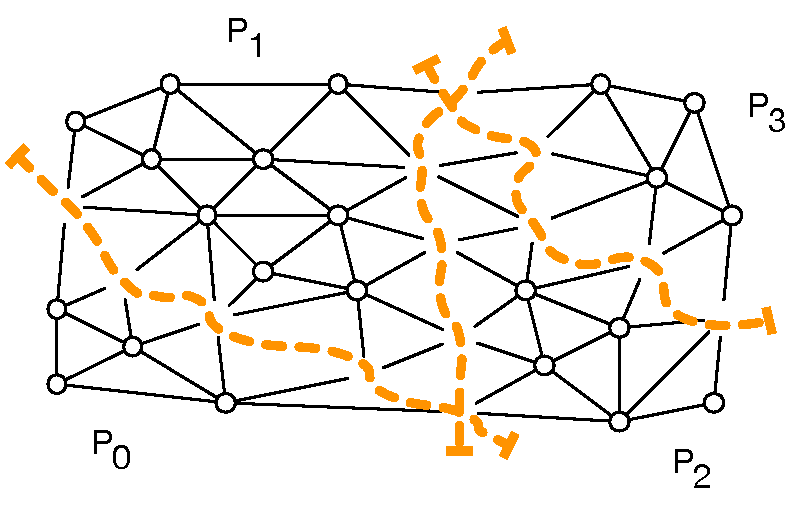
\includegraphics[scale=0.7]{sparsetiling/figures/partiotioned.pdf}
\caption{Partitioning of the seed loop.}
\label{fig:st-initial-part-sm}
\end{figure}

In the later stages of the inspection, $T_i$ is populated with iterations from $L_1$ and $L_2$. The challenge in scheduling iterations from $L_j$ to $T_i$ is to guarantee that all data dependencies -- read after write, write after read, write after write -- are honored. In the next two sections, we use the running example to illustrate how iterations are assigned to tiles to enable shared-memory and distributed-memory parallelism.

The result of the inspection is eventually passed to the executor. The inspection carries sufficient information for a parallel computation of different tiles. A given tile $T_i$ is always executed by a single thread/process ``atomically''; that is, without ever communicating with other threads/processes. When executing $T_i$, first all iterations from $L_0$ are executed, then all iterations from $L_1$ and finally those from $L_2$.

\subsection*{Inspection for Shared-Memory Parallelism}
\label{sec:tiling:ex-sm}
Similarly to OP2, to achieve shared-memory parallelism we use coloring. Two tiles that are given the same color can be executed in parallel by different threads. Two tiles can have the same color if they are not connected, because this ensures the absence of race conditions through indirect memory accesses during parallel execution. In the example we can use three colors: red (R), green (G), and blue (B). $T_0$ and $T_3$ are not connected, so they are assigned the same color. The colored tiles are shown in Figure~\ref{fig:st-loop-0}. In the following, with the notation $T_i^c$ we indicate that the $i$-th tile has color $c$. 

\begin{figure}[b]
\centering
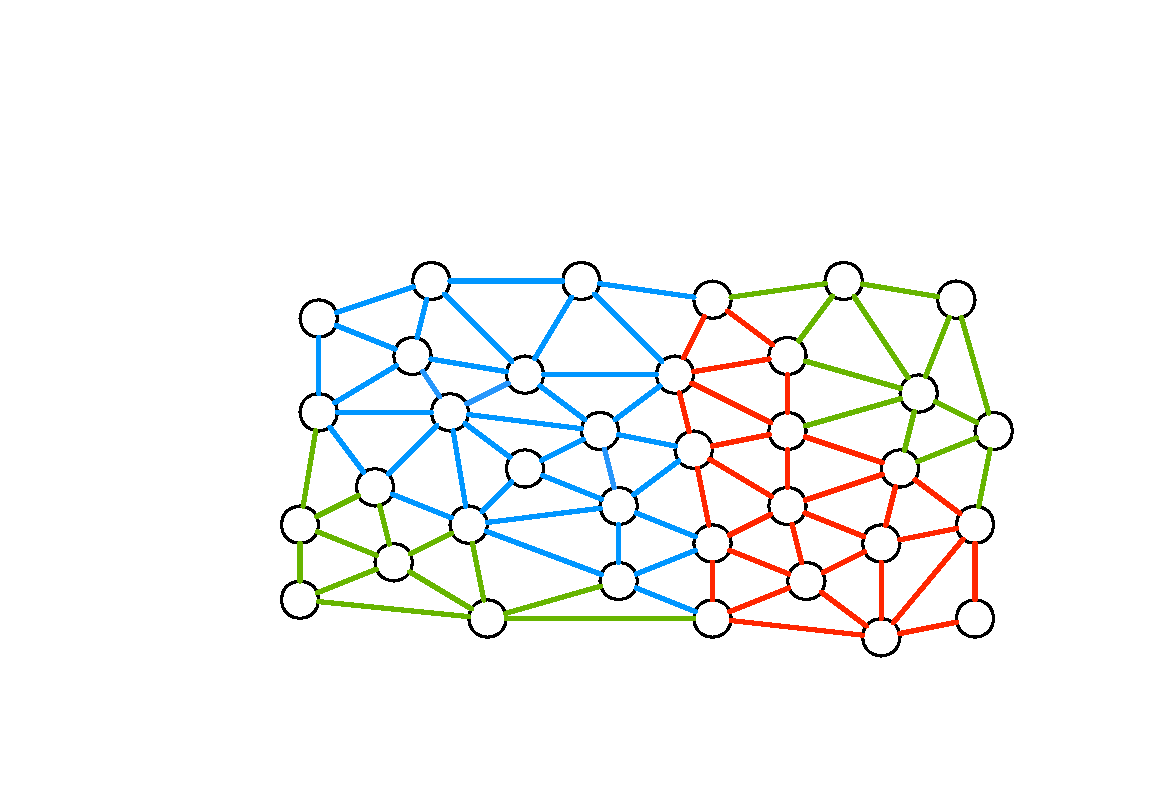
\includegraphics[scale=0.7]{sparsetiling/figures/loop_0.pdf}
\caption{Tiling $L_0$.}
\label{fig:st-loop-0}
\end{figure}

To populate the tiles with iterations from $L_1$ and $L_2$, we first have to establish a total ordering for the execution of partitions with different colors. Here, we assume the following order: green (G), blue (B), and red (R). This means, for instance, that \textit{all iterations} assigned to $T_1^B$ must be executed \textit{before all iterations} assigned to $T_2^R$. By ``all iterations'' we mean the iterations from $L_0$ (determined by the seed partitioning) as well as the iterations that will later be assigned from $L_1$ and $L_2$. We assign integer positive numbers to colors to reflect their ordering, where a smaller number means higher execution priority. In this case, we can assign 0 to green, 1 to blue, and 2 to red.


\begin{figure}[h]
\centering
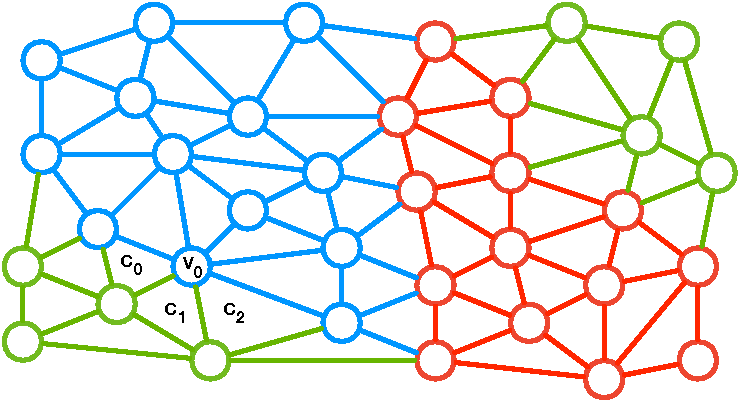
\includegraphics[scale=0.7]{sparsetiling/figures/loop_0_with_vertices.pdf}
\caption{Projection of $L_0$ to $L_1$.}
\label{fig:st-loop-0-proj}
\end{figure}

\begin{figure}[h]
\centering
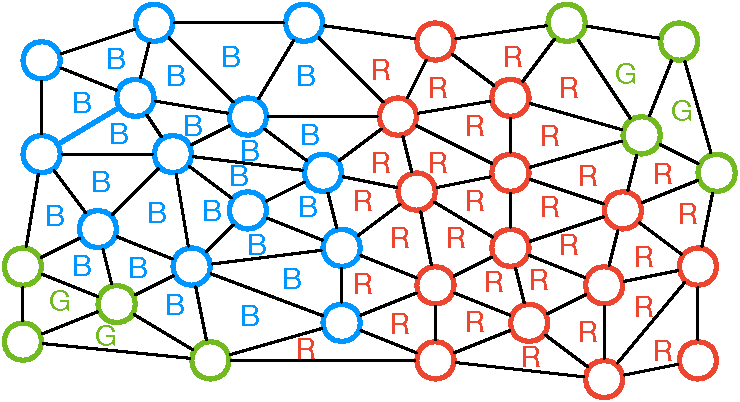
\includegraphics[scale=0.7]{sparsetiling/figures/loop_1.pdf}
\caption{Tiling $L_1$.}
\label{fig:st-loop-1}
\end{figure}

To schedule the iterations of $L_1$ to $[T_0^G,\ T_1^B,\ T_2^R,\ T_3^G]$, we first need to compute a \textit{projection} of any write or local reduction performed within $L_0$.  A projection for $L_0$ is a function $\phi : V \rightarrow \mathbb{T}$ mapping a vertex indirectly incremented during the execution of $L_0$ (see Listing~\ref{code:tiling-runningexample}) to a tile. Consider the vertex $v_0$ in Figure~\ref{fig:st-loop-0-proj}. $v_0$ has 7 incident edges, 2 of which belong to $T_0^G$, while the remaining 5 to $T_1^B$. Since we established that $G \prec B$, $v_0$ can only be read after $T_1^B$ has finished executing the iterations from $L_0$ (i.e., the 5 incident blue edges). We express this condition by setting $\phi(v_0) = T_1^B$. Observe that we can compute $\phi$ by iterating over $V$ and, for each vertex, applying the maximum function ($MAX$) to the color of the adjacent edges. 

We now use $\phi$ to schedule $L_1$, a loop over cells, to the tiles. Consider again $v_0$ and the adjacent cells $[c_0,\ c_1,\ c_2]$. These three cells have in common the fact that they are adjacent to both green and blue vertices. For $c_1$, and similarly with the other cells, we compute $MAX(\phi(v_0),\ \phi(v_1),\ \phi(v_2)) = MAX(B, G, G) = B = 1$. This establishes that $c_1$ must be assigned to $T_1^B$, because otherwise ($c_1$ assigned instead to $T_0^G$) a read to $v_0$ would occur before the last increment from $T_1^B$ took place. We indeed reiterate once more that the execution order is ``all iterations from $[L_0, L_1, L_2]$ in the green tiles before all iterations from $[L_0, L_1, L_2]$ in the blue tiles''. The result of scheduling $L_1$ to tiles is displayed in Figure~\ref{fig:st-loop-1}.

To schedule $L_2$ to $[T_0^G,\ T_1^B,\ T_2^R,\ T_3^G]$ we employ a similar process. Vertices are again written by $L_1$, so a new projection over $V$ will be computed and will be used in place of $\phi$ to schedule the edges in $L_2$. Figure~\ref{fig:st-loop-2} shows the result of this last phase. 

\begin{figure}[h]
\centering
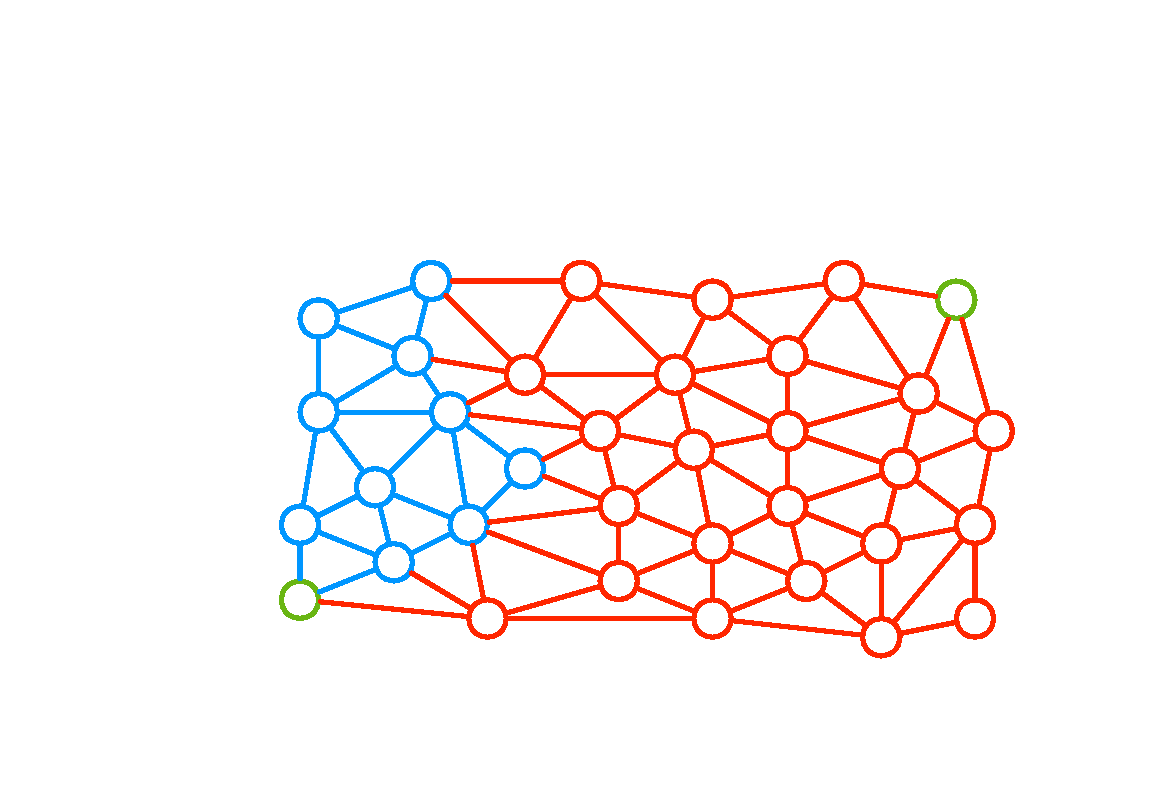
\includegraphics[scale=0.7]{sparsetiling/figures/loop_2.pdf}
\caption{Tiling $L_2$.}
\label{fig:st-loop-2}
\end{figure}


\subsubsection*{Conflicting Colors}
It is worth noting how $T_2^R$ ``consumed'' the frontier elements of all other tiles every time a new loop was scheduled. Tiling a loop chain consisting of $k$ loops had the effect of expanding the frontier of a tile of at most $k$ vertices. With this in mind, we re-inspect the loop chain of the running example, although this time with different execution order -- blue (B), red (R), and green (G) -- and initial partitioning. We recall that the total ordering of colors is indeed arbitrary. By applying the same inspection procedure that we just described, $T_0^G$ and $T_3^G$ will eventually become connected (see Figure~\ref{fig:st-conflicts}), thus violating the precondition ``tiles/partitions with the same color can run in parallel''. Race conditions during the execution of iterations belonging to $L_2$ are now theoretically possible. We will solve this problem in Section~\ref{sec:tiling:inspector}.

\begin{figure}[h]
\centering
\begin{subfigure}[b]{0.33\textwidth}
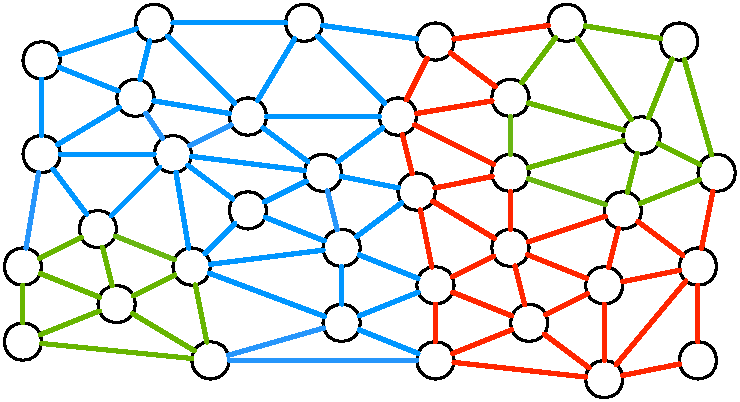
\includegraphics[width=\textwidth]{sparsetiling/figures/loop_0_conflicts.pdf}
\caption{After tiling $L_0$}
\label{fig:st-conflicts-a}
\end{subfigure}%
~ 
\begin{subfigure}[b]{0.33\textwidth}
\centering
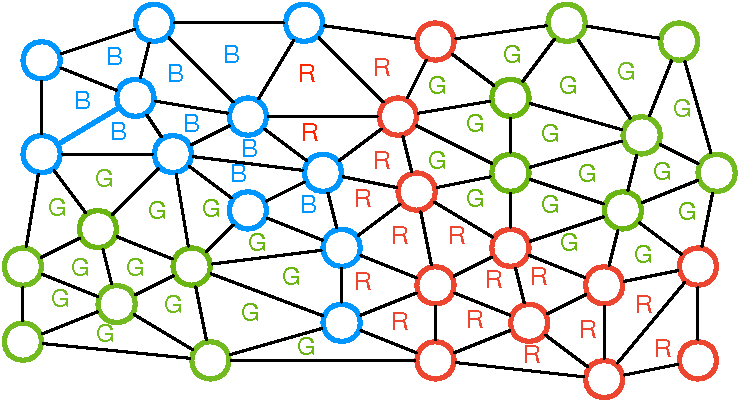
\includegraphics[width=\textwidth]{sparsetiling/figures/loop_1_conflicts.pdf}
\caption{After tiling $L_1$}
\label{fig:st-conflicts-b}
\end{subfigure}%
~
\begin{subfigure}[b]{0.34\textwidth}
\centering
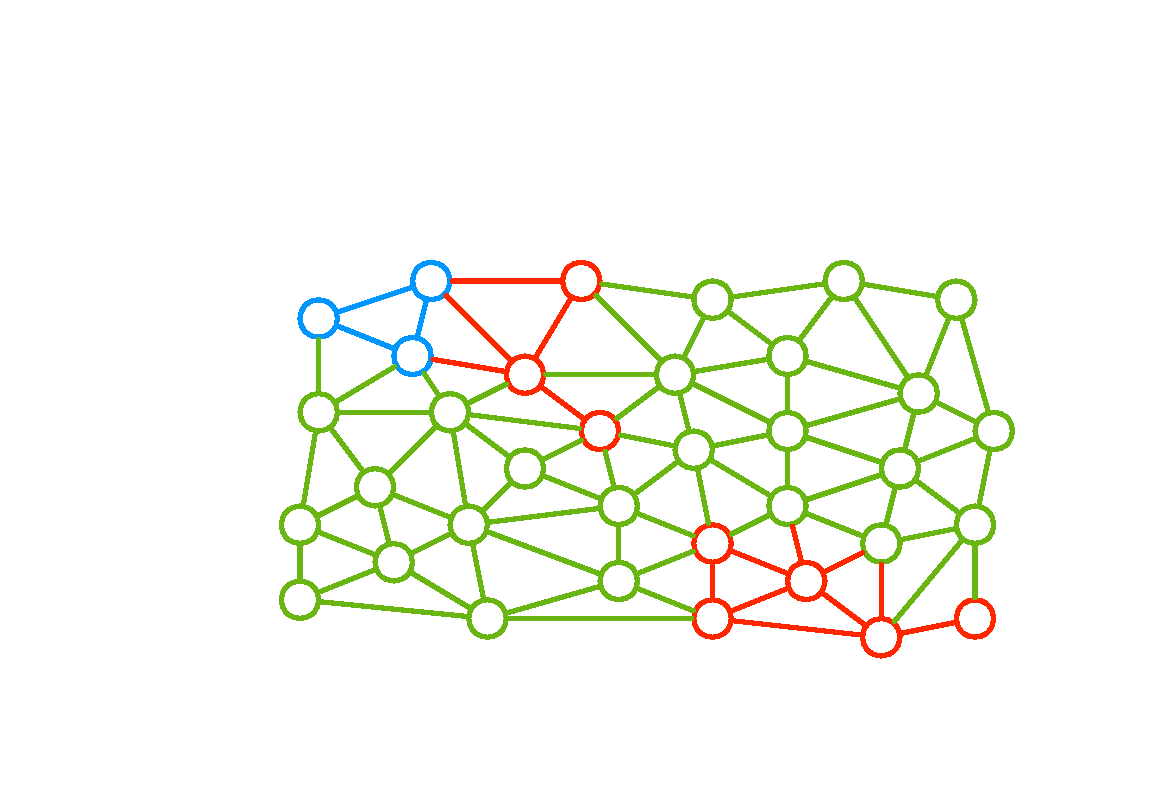
\includegraphics[width=\textwidth]{sparsetiling/figures/loop_2_conflicts.pdf}
\caption{After tiling $L_2$}
\label{fig:st-conflicts-c}
\end{subfigure}%

\caption{Tiling the program in Listing~\ref{code:tiling-runningexample} for shared memory parallelism can lead to conflicts. Here, the two green tiles eventually become adjacent, exposing potential race conditions.}
\label{fig:st-conflicts}
\end{figure}

\subsection*{Inspection for Distributed-Memory Parallelism}
\label{sec:tiling:ex-dist}
If parallelism is achieved through message-passing, the mesh and its datasets are distributed to different processes. Similarly to the example in Listing~\ref{code:tiling-struct}, MPI calls now separate the execution of two consecutive loops in the chain. This means that our inspector/executor scheme will have to take extra care of data dependencies along the mesh partition boundaries.

From Section~\ref{sec:tiling:lc-unstruct} we know that all sets are logically split into three regions, \textit{core}, \textit{boundary}, and \textit{non-exec}. The boundary region includes all iterations that cannot be executed until the MPI communications have successfully been accomplished. With this in mind, we take again $L_0$ as seed loop and make the following adjustments to the procedure illustrated in the previous section:
\begin{enumerate}
\item We take the core region of $L_0$ and partition it into tiles. Unless we aim for a mixed distributed/shared-memory parallelization scheme, there is no need to reassign the same color to unconnected tiles since we now have a single process executing sequentially a group of tiles . We can assign colors increasingly: $T_i$ is given color $i$. This allows us to uniquely identify a tile's color with its index, $i$. As long as tiles with contiguous ID are also physically contiguous in the mesh, this assignment retains spatial locality when ``jumping'' from executing $T_i$ to $T_{i+1}$.
\item We replicate for the boundary region of $L_0$ what we just did for the core. By neatly separating the core and boundary regions, we prevent tiles from crossing the two regions by construction. Further, all tiles within boundary have greater color than those in core, which poses a constraint on the execution order: no boundary tiles can be executed until all core tiles have been scheduled.
\item We map the whole non-exec region of $L_0$ to a single special tile, $T_{ne}$. This tile has highest color and will actually never be executed. Its role will be explained in later sections.
\end{enumerate}

In Figure~\ref{fig:st-mpi-init}, the same mesh of Figure~\ref{fig:st-initial-part-sm} has been distributed to two processes and the output of the initialization phase is displayed. The inspection then proceeds as in the case of shared memory parallelism. The application of the $MAX$ function when scheduling iterations from $L_1$ and $L_2$ to tiles makes higher color tiles (i.e., those that will be scheduled later at execution time) ``grow over'' lower color ones. The whole boundary region ``expands'' over core, and so does $T_{ne}$ over boundary (see Figure~\ref{fig:st-mpi-growth}). 

\begin{figure}[h]
\centering
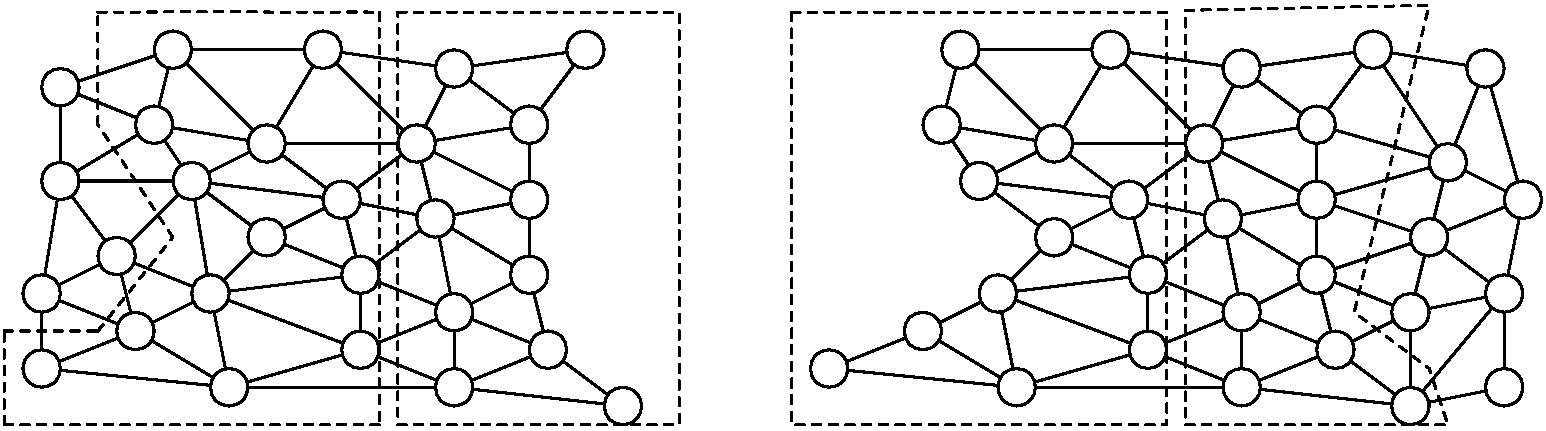
\includegraphics[width=\textwidth]{sparsetiling/figures/base_mesh_doppio.pdf}
\caption{Seed partitioning for distributed memory execution.}
\label{fig:st-mpi-init}
\end{figure}

On each process, the executor starts with triggering the MPI communications required for the execution of (all tiles over) the boundary regions; it proceeds to scheduling the core tiles, thus overlapping communication with computation; eventually, as soon as all core tiles have been executed and the MPI communications been accomplished, it computes the boundary tiles.

Finally, we observe that:
\begin{description}
\item[Correctness] This inspector/executor scheme relies on redundant computation along the boundaries of mesh partitions. The depth of the boundary region -- a parameter of the loop chain, as explained in Section~\ref{sec:tiling:lc-unstruct} -- grows proportionally with the number of loops that are fused. Roughly speaking, if the loop chain consists of $n$ loops, then the boundary region needs $n-1$ extra layers of elements. In Figure~\ref{fig:st-mpi-init}, the elements $[...]$ belong to $R_1$, although they also need be executed by $R_0$ in order for $[...]$ to be correctly computed when $T_x$ executes iterations from $L_2$. This is a conceptually simple expedient, although it poses a big challenge on software engineering. 
\item[Efficiency] The underlying hypothesis is that the increase in data locality achieved through sparse tiling will outweigh the overhead introduced by the redundant computation. This is based on the consideration that, in real applications, the core region tends to be way larger than the boundary one. In addition, not all iterations along the boundary region need be redundantly executed at every loop. For example, if we consider Figure~\ref{fig:st-mpi-nonexec}, we see that the strip of elements $[...]$ is not relevant any more for the correct computation of $[...]$. The non-exec tile $T_{ne}$, which we recall is not scheduled by the executor, is deliberately given the highest color to grow over the boundary region: this will leave dirty values in some datasets until the next round of MPI communications, but will not hurt correctness. 
\end{description}



%The main difference with respect to frameworks such as OP2 (see Section~\ref{sec:bkg:op2}) is that here, for reasons that will be more evident next, two regions, \textit{owned} and \textit{exec}, have been merged into a single one, \textit{boundary}. In essence, 


\section{Formalization}
\label{sec:tiling:algo}

\subsection{Data Dependency Analysis for Loop Chains}

As with all loop optimizations that reschedule the iterations in a sequence of loops, any sparse tiling must satisfy the data dependencies. The loop chain abstraction, which we have described in Section~\ref{sec:tiling:lc}, provides enough information to construct an inspector which analyzes all of the dependencies in a computation and builds a legal sparse tiling. We recall that one of the main assumptions in a loop chain is that each loop is fully parallel or, equivalently, that there are no loop carried dependencies.

The descriptors in the loop chain abstraction enable a general derivation of the storage-related dependencies between loops in a loop chain. The storage related dependencies between loops can be described as either flow (read after write), anti (write after read), or output (write after write) dependencies. In the following, assume that loop $L_x$, having iteration space $S_x$, always comes before loop $L_y$, having iteration space $S_y$, in the loop chain. Let us identify a descriptor of a loop $L$ with $m_{S_i \rightarrow S_j}^{mode}$: this simply indicates that the loop $L_i$ has iteration space $S_i$ and uses a map $m$ to write/read/increment elements (respectively, $\texttt{mode} \in \lbrace w, r, i\rbrace$) in the space $S_j$.

The flow dependencies can then be enumerated by considering pairs of points ($\vec{i}$ and $\vec{j}$) in the iteration spaces of the two loops $L_x$ and $L_y$:
\[
	\{ \vec{i} \rightarrow \vec{j} \; | \; \vec{i} \in S_x \wedge \vec{j} \in S_y \wedge 
	m_{S_x\rightarrow S_z}^{w}(\vec{i}) \cap m_{S_y \rightarrow S_z}^{r}(\vec{j}) \ne \emptyset \}.
\]
Anti and output dependencies are defined in a similar way. The anti dependencies for all pairs of loops $L_x$ and $L_y$ are:
\[
	\{ \vec{i} \rightarrow \vec{j} \; | \; \vec{i} \in S_x \wedge \vec{j} \in S_y \wedge 
	m_{S_x\rightarrow S_z}^{r}(\vec{i}) \cap m_{S_y \rightarrow S_z}^{w}(\vec{j}) \ne \emptyset \}.
\]
While the output dependencies between loops $L_x$ and $L_y$ are:
\[
	\{ \vec{i} \rightarrow \vec{j} \; | \; \vec{i} \in S_x \wedge \vec{j} \in S_y \wedge 
	m_{S_x\rightarrow S_z}^{w}(\vec{i}) \cap m_{S_y \rightarrow S_z}^{w}(\vec{j}) \ne \emptyset \}.
\]
In essence, there is a storage-related data dependence between two iterations from different loops (and therefore between the tiles they are placed in) when one of those iterations writes to a data element and the other iteration reads from or writes to the same data element.

There are local reductions, or ``reduction dependencies'' between two or more iterations of the same loop when those iterations ``increment'' the same location(s); that is, when they read, modify with a commutative and associative operator, and write to the same location(s). The reduction dependencies in $L_x$ are:
\[
	\{ \vec{i} \rightarrow \vec{j} \; | \; \vec{i} \in S_x \wedge \vec{j} \in S_x \wedge m_{S_x\rightarrow S_z}^{i}(\vec{i}) \cap m_{S_x \rightarrow S_z}^{i}(\vec{j}) \ne \emptyset \}.
\]
The reduction dependencies between two iterations within the same loop indicates that those two iterations must be executed atomically with respect to each other.

As seen in the example in Section~\ref{sec:tiling:ex-sm}, our inspector algorithm handles data dependencies, including those between non-adjacent loops, by tracking \textit{projections}. In the next section we explain how projections are constructed and used.

%In order to schedule $L$ to tiles, an up-to-date projection for each set $S$ accessed by $L$ must be available. For example, assume that $S$ is read by $L_k$ and is written by both $L_i$ and $L_j$. In the loop chain, the loops are in the order $L_i \prec ... \prec L_j \prec ... \prec L_k$. Let us denote by $\phi_S$ the projection for $S$. Each time that a loop accessing $S$ in write mode is inspected for scheduling, $\phi_S$ must be updated. When eventually scheduling $L_k$, therefore, an up-to-date snapshot of $\phi_S$ (i.e., the one produced right after tiling $L_j$) will be used to compute a legal tiling.


\subsection{The Generalized Sparse Tiling Inspector}
\label{sec:tiling:inspector}

The pseudo-code for the generalized sparse tiling inspector is showed in Algorithm~\ref{algo:st-inspector}. Given a loop chain and an average tile size, the algorithm produces a schedule suitable for mixed distributed/shared memory parallelism. In the following, we elaborate on the main steps of the algorithm. The notation used throughout the section is summarized in Table~\ref{table:st-summary-notation}.

\begin{table}
\centering
\begin{tabulary}{1.0\columnwidth}{C|C}
\hline
Symbol & Meaning \\
\hline
$\mathbb{L}$ & The loop chain \\
$L_i$ & The $i$-th loop in $\mathbb{L}$ \\ 
$S_i$ & The iteration space of $L_i$ \\
$S_i^{c}$, $S_i^{b}$, $S_i^{n}$ & the core, boundary, and non-exec regions of $S_i$ \\ 
$S$ & A generic set in $\mathbb{L}$ \\
$S_{in}$, $S_{out}$ & The input and output sets of a map \\
$D$ & A descriptor of a loop \\
$r$, $w$, $i$ & Possible values for $D$.mode \\
$\mathbb{T}$ & The set of all tiles \\
$\mathbb{T}[i]$ & Accessing the $i$-th tile \\
$T_i^{c}$, $T_i^{b}$ & the $i$-th tile over the core and boundary regions \\
$\phi_S$ & A projection $\phi_S : S \rightarrow \mathbb{T}$ \\
$\Phi$ & The set of all available projections \\
$\sigma_i$ & The tiling function $\sigma_i : S_i \rightarrow \mathbb{T}$ for $L_i$ \\
\hline
\end{tabulary}
\caption{Summary of the notation used throughout the section.}
\label{table:st-summary-notation}
\end{table}

\setcounter{algocf}{0}% Modify counter of algorithm
\begin{algorithm}[t]
\kwInput{The loop chain $\mathbb{L} = [L_0,\ L_1,\ ...,\ L_{n-1}]$, a tile size $ts$}
\kwOutput{A set of tiles $\mathbb{T}$, populated with iterations from $\mathbb{L}$}
\nonl ~\\
\Comment{Initialization}
$seed \gets 0$\;
$\Phi \gets \emptyset$\;
$C \gets \perp$\;
\nonl ~\\
\Comment{Creation of tiles}
$\sigma_{seed}$, $\mathbb{T} \gets$ partition($S_{seed}$, $ts$)\;
seed$\_$map $\gets$ find$\_$map($S_{seed},\ \mathbb{L}$)\;
conflicts $\gets$ false\;
\nonl ~\\
\Comment{Schedule loops to tiles}
\Do{conflicts}{
  color($\mathbb{T}$, seed$\_$map)\;
   \nonl ~\\
  \For{$i=1$ \KwTo $n-1$}{
    project($L_{i-1}$, $\sigma_{i-1}$, $\Phi$, $C$)\;
    $\sigma_i \gets$ tile($L_i$, $\Phi$)\;
    assign($\sigma_i$, $\mathbb{T}$)\;
  }
  \nonl ~\\
  \If{found$\_$conflicts($C$)}{
    conflicts $\gets$ true\;
    add$\_$fake$\_$connection(seed$\_$map, $C$)\;
  }
}
\nonl ~\\
\Comment{Inspection successful, create local maps and return}
create$\_$local$\_$maps($\mathbb{T}$)\;
\Return{$\mathbb{T}$}
\caption{The inspection algorithm}
\label{algo:st-inspector}
\end{algorithm}




\paragraph{Choice of the seed loop}
The seed loop $L_{seed}$ is used to initialize the tiles. Theoretically, any loop in the chain can be chosen as seed. Supporting distributed memory parallelism, however, is cumbersome if $L_{seed} \neq L_0$. This is because more general partitioning and coloring schemes would be needed to ensure that no iterations in any $S_i^{b}$ are assigned to a core tile. A constraint of our inspector algorithm in the case of distributed memory parallelism is that $L_{seed} = L_0$. 

In the special case in which there is no need to distinguish between core and boundary tiles (because a program is executed on a single shared-memory system), the seed loop can be chosen arbitrarily. If we however pick $L_{seed}$ in the middle of the loop chain ($L_0 \prec ... \prec L_{seed} \prec ...$), a mechanism for constructing tiles in the reverse direction (``backwards''), from $L_{seed}$ towards $L_0$, is necessary. In~\cite{st-paper}, we propose two ``symmetric'' algorithms to solve this problem, \textit{forward tiling} and \textit{backward tiling}, with the latter using the $MIN$ function in place of $MAX$ when computing projections. For ease of exposition, and since in the fundamental case of distributed memory parallelism we impose $L_{seed} = L_0$, we here neglect this distinction\footnote{The algorithm that is implemented in the SLOPE library, however, is more general and supports backwards tiling for the case in which distributed memory parallelism is not required.}. 

%\textit{Note: in real applications loops over ``subsets'' are possible; for instance, a loop over the exterior facets of the mesh. If one such loop is picked as seed, then the inspection is aborted.}

\paragraph{Tiles initialization}
The algorithm starts with partitioning $S_{seed}^{c}$ into $m$ subsets $\lbrace P_0, P_1, ..., P_{m-1}\rbrace$ such that $P_i \cap P_j = \emptyset$ and $\cup_{i = 0}^{m-1} P_i = S_{seed}^{c}$. The partitioning is sequential: $S_{seed}$ is ``chunked'' every $ts$ iterations, with $P_{m-1}$ that may be smaller than all other partitions. Similarly, we partition $S_{seed}^{b}$ into $k$ subsets.

We then create $m+k+1$ tiles, $\mathbb{T} = \lbrace T_0^c, ..., T_{m-1}^c, T_m^{b}, ..., T_{m+k-1}^b, T_{m+k}^{n} \rbrace$, one for each partition and one extra tile for $S_{seed}^{n}$. 

A tile $T_i$ has four fields, as summarized in Table~\ref{table:st-tile-structure}. The region is used by the executor to schedule tiles in a certain order. The value of this field is determined right after the seed partitioning, since a tile is exclusively in one of $\lbrace S_{seed}^c, S_{seed}^b, S_{seed}^n \rbrace$. The iterations lists represent the iterations in $\mathbb{L}$ belonging to $T_i$. For each $L_j \in \mathbb{L}$, there is one iterations list $T_i^{L_j}$. At the beginning, for each $T_i \in \mathbb{T}$ we have $T_i^{L_{seed}} = T_i^{L_0} = P_i$, whereas all other lists are empty. Local maps are used by the executor in place of the global maps provided by the loop chain; we will see that this allows avoiding double indirections.


\begin{table}
\centering
\begin{tabulary}{1.0\columnwidth}{P{2.7cm} | P{8.5cm}}
\hline
Field & Possible values \\
\hline
region & core, boundary, non-exec \\
color & an integer representing the execution priority \\ 
iterations lists & one list of iterations (integers) $T_i^{L_j}$ for each $L_j \in \mathbb{L}$\\ 
local maps & one list of local maps for each $L_j \in \mathbb{L}$; one local map for each map used in $L_j$\\
\hline
\end{tabulary}
\caption{The tile data structure.}
\label{table:st-tile-structure}
\end{table}

Each tile needs be assigned a color, which gives it a scheduling priority. If shared memory parallelism is requested, adjacent tiles are given different colors (the adjacency relation is determined through the maps available in $\mathbb{L}$). Otherwise, the colors are assigned to the tiles in increasing order (i.e., $T_i$ is given color $i$). The boundary tiles are always given colors higher than that of core tiles; the non-exec tile has highest color. In essence, this will allow the executor to schedule all core tiles first and all boundary tiles afterwards. 

\paragraph{Construction of tiles by tracking data dependencies}
To schedule a loop to tiles we use projections. A projection is a function $\phi_S : S \rightarrow \mathbb{T}$. Projections are computed and/or updated after tiling a loop. Initially, the set $\Phi$ of all projections is empty. Starting with the seed tiling $\sigma_{seed} : S_{seed} \rightarrow \mathbb{T}$, we iteratively update $\Phi$ and build tiling functions for all other loops $[L_1, L_2, ..., L_{n-1}]$. 

\paragraph{Projecting tiled sets}

\begin{algorithm}[t]
\kwInput{A loop $L_{i}$, a tiling function $\sigma_{i}$, the projections set $\Phi$, the conflicts matrix $C$}
\KwResult{Update $\Phi$ and $C$}
\nonl ~\\
\ForEach{$D$ in $L_i$.descriptors}{
  \If{$D$.mode $==$ r}{
    skip\;
  }
  \eIf{$D$.map $== \perp$}{
    $\Phi = \Phi \cup \sigma_{i}$\;
  }{
    inverse$\_$map $\gets$ map$\_$invert($D$.map)\;
    $S_{j}$, $S_{i}$, values, offsets $\gets$ inverse$\_$map\;
    $\phi_{S_{j}} \gets \perp$\; 
    \For{$e=0$ \KwTo $S_j$.size}{ \label{algo:st-projection-parallel}
      \For{$k=$ offsets[e] \KwTo offsets[e+1]}{
        adjacent$\_$tile = $\mathbb{T}$[values[k]]\;
        max$\_$color $\gets$ MAX($\phi_{S_{j}}[e]$.color, adjacent$\_$tile.color)\;
        \If{max$\_$color $\neq$ $\phi_{S_{j}}[e]$.color}{
          $\phi_{S_{j}}[e] \gets$ adjacent$\_$tile\;
        }
      }
    }
    update($C$, $\mathbb{T}$, $\phi_{S_{j}}$)\;
    $\Phi = \Phi \cup \phi_{S_{j}}$\;
  }
}
\caption{Projection of a tiled loop}
\label{algo:st-projection}
\end{algorithm}

Algorithm~\ref{algo:st-projection} takes as input $\sigma_{i-1}$ and (the descriptors of) $L_{i-1}$ to update $\Phi$. Further, the conflicts matrix $C \in \mathbb{N}^{m \times m}$, indicating whether two different tiles having the same color will become adjacent after tiling $L_{i-1}$, is updated. 

A projection tells what tile a set element logically belongs to at a given point of the tiling process. A new projection $\phi_{S}$ is needed if the elements of $S$ are written by $L_i$. Let us consider the non-trivial case in which writes or increments occur indirectly through a map $M : S_i \rightarrow S_j^0 \times S_j^1 \times ... \times S_j^{a-1}$. To compute $\phi_{S_{j}}$, we first determine the inverse map (an example is shown in Figure~\ref{fig:st-inverse-map}). Then, we iterate over all elements of $S_i$ that indirectly access elements in $S_j$. In particular, given $e \in S_j$, we determine the last tile that writes to $e$, say $T_{last}$, through the application of the $\operatorname{MAX}$ function to tile colors. We then simply set $\phi_{S_{j}}[e] = T_{last}$. 


% ($C[i,j] = 1$ implies that $T_i$ and $T_j$ have the same color and will become adjacent after tiling $L_{i-1}$).

\paragraph{Scheduling loops} 

\begin{algorithm}[t]
\kwInput{A loop $L_{i}$ (with iteration space $S_i$), the projections set $\Phi$}
\kwOutput{The tiling function $\sigma_{i}$}
\nonl ~\\
$\sigma_i \gets \perp$\;
\ForEach{$D$ in $L_i$.descriptors}{
  \eIf{$D$.map $== \perp$}{
    $\sigma_i \gets \Phi[S_i]$\;    
  }{
    arity $\gets D$.map.arity\;
    $\phi_{S} \gets \Phi[D$.map.$S_{j}$]\;
    \For{$e=0$ \KwTo $S_i$.size}{ \label{algo:st-tiling-parallel}
       $\sigma_i[e] \gets T_{\perp}$ \;
      \For{$k=0$ \KwTo arity}{
        adjacent$\_$tile $\gets \phi_{S}$[$D$.map.values[e*arity + k]]\;
        max$\_$color $\gets$ MAX($\sigma_i[e]$.color, adjacent$\_$tile.color)\;
        \If{max$\_$color $\neq$ $\sigma_i[e]$.color}{
          $\sigma_i[e] \gets$ adjacent$\_$tile\;
        }
      }
    }
  }
}
\Return{$\sigma_i$}
\caption{Building a tiling function}
\label{algo:st-tiling}
\end{algorithm}

Using $\Phi$, we compute $\sigma_i$ as described in Algorithm~\ref{algo:st-tiling}. The algorithm is similar to the projection of a tiled loop, with the main difference being that now we use $\Phi$ to schedule iterations correctly. Finally, $\sigma_i$ is inverted and the iterations added to the corresponding iteration lists $T_j^{L_i}$ of all $T_j \in \mathbb{T}$. 


\paragraph{Detection of conflicts}
If $C$ indicates the presence of at least one conflict, say between $T_i$ and $T_j$, we add a ``fake connection'' between $T_i$ and $T_j$ and loop back to the coloring stage. $T_i$ and $T_j$ are now connected, so they will receive different colors. 
%Otherwise, a legal tiling has now been computed. 



\subsection{The Generalized Sparse Tiling Executor}

\begin{algorithm}[t]
\kwInput{A set of tiles $\mathbb{T}$}
\KwResult{Execute the loop chain, thus modifying the data sets written or incremented within $\mathbb{L}$}
\nonl ~\\
$\mathbb{T}^{c}$, $\mathbb{T}^{b}$ $\gets$ group$\_$tiles$\_$byregion($\mathbb{T}$)\;
\nonl ~\\
start$\_$MPI$\_$communications()\;
\nonl ~\\
\ForEach{available color $c$}{
  \ForEach{$T \in \mathbb{T}^{c}$ s.t. $T$.color $== c$}{ \label{algo:st-executor:parallel1}
    execute$\_$tile($T$)\;
  }
}
\nonl ~\\
end$\_$MPI$\_$communications()\;
\nonl ~\\
\ForEach{available color $c$}{
  \ForEach{$T \in \mathbb{T}^{b}$ s.t. $T$.color $== c$}{ \label{algo:st-executor:parallel2}
    execute$\_$tile($T$)\;
  }
}
\caption{The executor algorithm}
\label{algo:st-executor}
\end{algorithm}


The sparse tiling executor is illustrated in Algorithm~\ref{algo:st-executor}. It consists of four main phases: triggering of MPI communications; execution of core tiles (in overlap with communication); waiting for the termination of all MPI communications; execution of boundary tiles.

As seen in the example in Section~\ref{sec:tiling:ex-dist} and based on the explanation in Section~\ref{sec:tiling:inspector}, we know that the core tiles do not require any off-process information to execute as long as the boundary regions are (i) up-to-date and (ii) ``sufficiently deep''. If both conditions hold, the execution is semantically correct and it is safe to overlap computation of core tiles with the communication of boundary data. 


\paragraph{The depth of the boundary region}
In $\mathbb{L}$ we have $n$ loops. A tile ``crosses'' all of these loops and is executed atomically; that is, once it starts executing its iterations, it reaches the end without the need for synchronization with other processes. With this execution model, the boundary region must include a sufficient amount of off-process iterations for a correct computation of the tiles along the border with the core region. 

In the extreme case $n=1$, a single ``strip'' of iterations belonging to adjacent processes need be redundantly executed. As $n$ increases, more off-process data is required. If $n=3$, as in the example in Figure~\ref{fig:tiling:mpi-n3}, we need three ``strips'' of off-process iterations to be computed in order for the datasets over $X$ to be correctly updated when executing iterations belonging to $L_3$.

The {\em depth} is a parameter provided through the loop chain abstraction that informs the inspector about the extent of the boundary region. For correctness, we cannot tile more than {\em depth} loops, so if $n >$ {\em depth} the loop chain must first be split into smaller sequences of loops, to be individually inspected and executed. 

%For ease of explanation, this aspect has been neglected in the inspector algorithms described in the previous section. 

%Our inspector/executor strategy, therefore, works correctly as long as the loop chain has been ``dimensioned'' properly, with sufficient information in all $S^{b}$ regions 

%\paragraph{The execution of a tile}


\subsection{Computational Complexity of Inspection}

\begin{table}[t]
\centering
\begin{tabulary}{1.0\columnwidth}{P{2.7cm} | c | c}
\hline
Phase & Cost shared memory & Cost distributed memory \\
\hline
Partitioning & $N$ & $N$ \\
Coloring & $R K $ & $N$ \\ 
Projection & $R (n M N K^2) $ & $n M N K^2 $ \\ 
Tiling & $R (n M N K) $ & $n M N K $ \\
Local maps & $n M$ & $n M$\\
\hline
\end{tabulary}
\caption{Worst-case costs of inspection.}
\label{table:st-comp-cost}
\end{table}

Let $N$ be the maximum size of a set in $\mathbb{L} = [L_0, L_1, ..., L_{n-1}]$ and let $M$ be the maximum number of sets accessed in a loop. If $a$ is the maximum arity of a map, then $K = a N$ is the maximum cost for iterating over a map. $K$ is also the worst-case cost for inverting a map. Let $p < 1$ be the probability that a conflict arises during inspection in the case of shared memory parallelism; thus, the expected number of inspection rounds is $R = \frac{1}{1-p}$. Hence, the worst-case computational costs of the main inspection phases are as in Table~\ref{table:st-comp-cost}.



%LOCAL MAPS: Finally, for each $T_i \in \mathbb{T}$, for each $L_j \in \mathbb{L}$, for each map used in $L_j$, create a local map. 

\section{Implementation}
\label{sec:tiling:automation}
The implementation of generalized sparse tiling is distributed over three software modules. 
\begin{description}
\item[Firedrake] This is the framework for the automated solution of finite element methods described in Section~\ref{sec:bkg:firedrake}. 
\item[PyOP2] Firedrake produces numerical kernels to be applied over sets of mesh components. The parallel iteration over the mesh is handled by PyOP2 (see Section~\ref{sec:bkg:op2}).
\item[SLOPE] A library for writing generalized inspector/executor schemes, with primary focus on sparse tiling. PyOP2 uses SLOPE for tiling loop chains.
\end{description}
The interaction among these modules is illustrated in Figure~\ref{fig:st-implementation}.

There are several reasons behind the choice of this three-layer structuring:
\begin{description}
\item[Simpler analysis] The abstractions used in Firedrake and PyOP2 simplify the analysis required for automation. For example, from the parallel loop construct in PyOP2 we can derive sufficient information to build a loop chain (see Section~\ref{sec:tiling:lc-unstruct}).
\item[User base] We wish generalized sparse tiling to be used in real scientific software, so we targeted a system with a user base in steady expansion. This increased the implementation effort, but it has also made sparse tiling promptly available to a wide audience.
\item[Flexibility] Adopting sparse tiling in a Firedrake program is the simplest option, because the generation of inspector/executor schemes is fully automated. If we instead have a PyOP2 program, the generation of inspector/executor schemes is only partly automated, since the separation of a set into the core, boundary and non-exec regions for distributed-memory parallelism must be coded explicitly. Users can also write an inspector-executor scheme from scratch, in which case the entire loop chain must be provided through direct calls to the SLOPE library (an example was provided in Listing~\ref{code:tiling-inspector}). This is clearly the most flexible yet complicated option. 
\end{description}


%- is automation possible ? -> DSLs !!! + lazy evaluation + inspector/executor + mpi-trick
% subsets ! seed loop cannot be subset

In the next sections, we describe the interplay between these three frameworks and how this leads to automation.

\subsection{SLOPE: a Library for Tiling Irregular Computations}
SLOPE is an open source software that provides a set of functions to build a loop chain and to write inspector/executor schemes for sparse tiling\footnote{SLOPE is freely available at \url{https://github.com/coneoproject/SLOPE}}. 

The loop chain abstraction implemented by SLOPE is the one described in Section~\ref{sec:tiling:lc-unstruct}. In essence, a loop chain comprises some sets (including the separation into core, boundary, and non-exec regions), maps between sets, and a sequence of loops. Each loop has one or more descriptors specifying what and how dataset are accessed. The example in Listing~\ref{code:tiling-inspection} illustrates the interface exposed by SLOPE for constructing loop chains. 

SLOPE implements all of the algorithms in Section~\ref{sec:tiling:inspector}. It also provides features to verify the effectiveness and the correctness of the transformations:
\begin{description}
\item[VTK file generator] For each tiled loop, a file showing the mesh and the repartition into colored tiles is generated. The file is suitable for visualization in Paraview~\cite{paraview}.
\item[The summary routine] The inspector returns useful information concerning the tiling process, including: the number and the average size of tiles, the total number of colors used (which can give an indication of how effective a shared-memory parallelization will be), times for the most critical inspection phases. 
\end{description}

In the case of shared-memory parallelism, the following sections of code are parallelized through OpenMP:
\begin{itemize}
\item The projection and tiling algorithms; in particular, the loop at line~\ref{algo:st-projection-parallel} of Algorithm~\ref{algo:st-projection} and the loop at line~\ref{algo:st-tiling-parallel} of Algorithm~\ref{algo:st-tiling}).
\item The execution of tiles having the same color; that is, the loops at lines~\ref{algo:st-executor:parallel1} and~\ref{algo:st-executor:parallel2} of Algorithm~\ref{algo:st-executor}.
\end{itemize}


\subsection{PyOP2: a Runtime Library for Mesh Iteration based on Lazy Evaluation}
PyOP2 has been described in Section~\ref{sec:bkg:op2}. This section focuses on three complementary aspects: (i) the interface with the user for identifying sequences of ``chainable'' loops; (ii) the lazy evaluation mechanism that allows building loop chains; (iii) the interface with SLOPE to run an inspector/executor scheme.

To trigger the creation of a loop chain, PyOP2 provides the {\em loop$\_$chain} construct. The use of this interface is exemplified in Listing~\ref{code:loop-chain-interface}. The {\em loop$\_$chain} interface is exposed to both users and higher layers of abstraction. Thus, in Firedrake we define a loop chain in a way analogous to PyOP2's, with the only difference being that loops are not visible in the source code because they are automatically generated from the mathematical notation.

The second fundamental aspect is that PyOP2 implements lazy evaluation of parallel loops. The parallel loops encountered or generated by Firedrake are first pushed into a queue. The sequence of parallel loops in the queue is called {\em trace}. If a field $f$ needs be read, for example because a user wants to inspect its values or a global linear algebra operation is about to be performed, the trace is traversed -- from the most recent parallel loop to the oldest one -- and a new sub-trace produced. The sub-trace, which includes all parallel loops that need be executed for a correct update of $f$, is finally executed. 

All loops in the trace that are created within a {\em loop$\_$chain} scope are sparse tiled through SLOPE. In detail, the interaction between PyOP2 and SLOPE is as follows:
\begin{enumerate}
\item As seen in the examples in Listing~\ref{code:loop-chain-interface}, the {\em loop$\_$chain} defines a new scope. As this scope is entered, a stamp $s_1$ of the loop chain is generated. This happens ``behind the scenes'', because the {\em loop$\_$chain} is a Python context manager, which executes pre-specified routines prior and after the execution of the body. As the {\em loop$\_$chain} is exited, a new stamp $s_2$ of the trace is computed, and all parallel loops generated between $s_1$ and $s_2$ are placed into a list for pre-processing.
\item The pre-processing consists of two main steps: ``simple'' fusion of all consecutive parallel loops iterating over the same iteration space that do not present read-after-write or write-after-read dependencies through indirections/maps; generation of a loop chain suitable for SLOPE.
\item SLOPE provides a thin Python interface to ease integration with other frameworks. PyOP2 inspects the sequence of loops and translates all relevant data structures (sets, maps, loops) into a format suitable for SLOPE. Eventually, a string of C code implementing an inspector for the loops in the {\em loop$\_$chain} is returned. PyOP2 just-in-time compiles this code and runs it, obtaining the {\em inspection} data structure.
\item A ``software cache'' mapping {\em loop$\_$chain}s to {\em inspection} data structures is used. This whole process is therefore executed only once for each unique {\em loop$\_$chain} encountered in the code. 
\item The executor is built analogously, and invoked each time a {\em loop$\_$chain} is exited.
\end{enumerate}

\subsection{Firedrake/DMPlex: the S-depth mechanism for MPI}
\label{sec:tiling:impl-firedrake}
Firedrake uses DMPlex~\citep{dmplex-cite} to handle meshes. In particular, DMPlex is responsible for partitioning, distributing over multiple processes, and locally reordering a mesh. The MPI parallelization, therefore, is completely handled in Firedrake.

During the start-up phase, each MPI process receives a contiguous partition of the original mesh from DMPlex. It then creates various PyOP2 sets, representing either mesh components (e.g., cells, vertices) or function spaces. As seen in Section~\ref{sec:bkg:op2}, PyOP2 sets distinguish between different regions: core, owned, exec, and non-exec. Firedrake is directly responsible for setting these regions and creating data structures enabling message passing among different processes.

To support our loop chain abstraction, Firedrake must be able to allocate arbitrarily deep halo regions; both Firedrake and DMPlex have been extended with this feature\footnote{Michael Lange carried out the bulk of the implementation.}. A parameter called {\em S-depth} (for historical reasons, see~\cite{s-depth-paper}), used for initializing a mesh, specifies the extent of the halo regions. A value of {\em S-depth} equal to $n$ indicates the presence of $n$ strips of off-process data elements in each set. The default value for {\em S-depth} is $1$, which corresponds to the standard execution model of Firedrake/PyOP2. Even in absence of sparse tiling, this value enables overlap of computation with communication, at the price of a small amount of redundant computation along partition boundaries.


\section{Performance Evaluation}
The experimentation was divided into two phases:

\begin{enumerate}
\item Generalized sparse tiling was initially applied to two benchmarks: a sparse Jacobi kernel and a proxy unstructured mesh application, originally developed as a demo for the OP2 framework. This was especially useful to identify strengths and limitations of the technique.
\item Then, it was used in an application developed in Firedrake, Seigen, an Elastic Wave Equation Solver for Seismological Problems\footnote{Seigen has been developed by Christian Jacobs.}. The aim of this phase was to evaluate the performance improvements in a real-world simulation.
\end{enumerate}

%note: tile size independent of mesh size !!!! but actually dependent on the application...!


\subsection{Benchmarks}
In this section, our objective is to explore the impact of generalized sparse tiling on performance, to characterize the circumstances where the approach is profitable, to identify the major limitations to a widespread adoption of the technique, and to justify some of the design choices made in the previous sections.

All benchmarks are written in C. The sparse tiled implementations only support shared memory parallelism via OpenMP. A previous version of the inspector algorithms presented in this chapter, described in~\cite{st-paper}, was used. As detailed next, one of the major drawbacks of this older inspector was its cost, which grew very rapidly with the number of loops in the chain and the number of distinct datasets accessed. 

In all the experiments presented in this section, the optimal tile size (i.e. the one leading to the best execution time) was determined empirically, for each combination of architecture and application. 

\subsubsection{Sparse Jacobi}

\begin{table}[t]
\centering
\begin{tabulary}{1.0\columnwidth}{c | c | c}
\hline
Matrix name & Execution time reduction & Speed-up  \\
\hline
{\em ldoor} & 40.34 & 12.11 \\
{\em pwtk} & 38.42 & 11.98 \\
{\em thermal2} & 25.78 & 11.08 \\
{\em xenon2} & 20.15 & 9.53 \\
{\em audikw$\_$1} & 13.42 & 8.70 \\
{\em nd24k} & -151.72 & 3.06 \\
\hline
\end{tabulary}
\caption{Execution time reductions over the original implementation (in percentage) and speed-ups over the single-threaded tiled implementation for the sparse Jacobi solver with 15 threads.}
\label{table:st-jacobi}
\end{table}

The first experiment was the full sparse tiling of a Jacobi sparse matrix solver\footnote{This section is partly extracted from~\cite{st-paper}, and the results were obtained from experiments conducted by Christopher D. Krieger, Catherine Olschanowsky, and Michelle Mills Strout}. Given a sparse matrix $A$, and a vector $\vec{f}$, related by $A\vec{u}=\vec{f}$, each iteration of the sparse Jacobi method produces an approximation to the unknown vector $\vec{u}$. In our experiments, the Jacobi convergence iteration loop is unrolled by a factor of two and the resulting two loops are chained together (1000 iterations of the loop chain was executed). Using a ping-pong strategy, each loop reads from one copy of the $\vec{u}$ vector and writes to the other copy. This experiment was run on an Intel Westmere (dual-socket 8-core Intel Xeon E7-4830 2.13 GHz, 24MB shared L3 cache per socket). The code was compiled using {\tt gcc-4.7.0} with options {\tt -O3 -fopenmp}.

The Jacobi recurrence equation includes a sparse matrix vector multiplication and is representative of a broad class of sparse linear algebra applications. It is also an effective test-bed because different data dependency patterns can be examined simply by using different input matrices. In these experiments, a set of 6 input matrices, drawn from the University of Florida Sparse Matrix Collection~\cite{ST-MatrixMarket}, was used. The matrices were selected so that they would vary in overall data footprint, from 45 MB to 892 MB, and in percentage of non-zeros, from very sparse at 0.0006\% to much more dense at 0.5539\% non-zeros. % values.

Table~\ref{table:st-jacobi} compares the performance of the tiled Jacobi solver to that of a simple blocked version. Both codes use OpenMP \texttt{parallel for} directives to achieve parallelism. The execution time reduction varied from 13$\%$ to 47$\%$ with the exception of the {\em nd24k} matrix, which showed as much as a 1.52x slowdown when sparse tiled. This matrix is highly connected, thus limiting the number of tiles that can be scheduled in parallel. The greater parallelism available under a blocked approach provides more benefit in this case than the performance improvements due to improved locality from full sparse tiling. Overall, speed-ups of between 8 and 12 times over the single-threaded tiled implementation were observed when using 15 threads; a clear outlier is again the {\em nd24k} matrix that did not scale past 3.2 times the single thread performance.

%and typically decreased as threads were added. We believe that this reduction is also related to the parallelism available in the task graph and are investigating methods to mitigate its impact.

The values in Table~\ref{table:st-jacobi} do not include the inspection time necessary to full sparse tile the loop chain. To break even when this cost is considered, the inspector time must be amortized over between 1000 and 3000 iterations of the executor, depending on the specific matrix being solved. We will further elaborate on this aspect in Section~\ref{sec:tiling:bench:conc}.



\subsubsection{Airfoil}


\begin{table}[t]
\centering
\begin{tabulary}{1.0\columnwidth}{c | c | c}
\hline
Implementation & Execution time & Speed-up \\
\hline
Westmere {\em omp} & 36.87 & 6.43\\
Westmere {\em mpi} & 31.0 & 7.66 \\
Westmere {\em tiled} & 26.49 & 8.96 \\
\hline \hline
Sandy Bridge {\em omp} & 30.01 & 6.65 \\
Sandy Bridge {\em mpi} & 24.42 & 8.17 \\
Sandy Bridge {\em tiled} & 20.63 & 9.67 \\
\hline
\end{tabulary}
\caption{Execution time (in seconds) and speed-ups over the slowest single-threaded implementation for the Airfoil benchmark. The values are obtained from simulations with fully-loaded machines (16 and 24 threads/processes on the Sandy Bridge and the Westmere architectures, respectively).}
\label{table:st-airfoil}
\end{table}

Airfoil is a representative unstructured mesh application~\cite{AIRFOIL}. Three implementations of Airfoil, {\em omp}, {\em mpi} and {\em tiled}, were compared on two shared-memory machines, an Intel Westmere (dual-socket 6-core Intel Xeon X5650 2.66 GHz, 12MB of shared L3 cache per socket) and an Intel Sandy Bridge (dual-socket 8-core Intel Xeon E5-2680 2.00Ghz, 20MB of shared L3 cache per socket). The code was compiled using the Intel \texttt{icc 2013} compiler with optimizations enabled (\texttt{-O3}, \texttt{-xSSE4.2/-xAVX}).

The Airfoil code consists of a main time loop with 2000 iterations. This loop contains a sequence of four parallel loops that carry out the computation. In this sequence, the first two loops, called $adt$-$calc$ and $res$-$calc$, constitute the bulk of the computation. $Adt$-$calc$ iterates over cells, reads from adjacent vertices and write to a local dataset, whereas $res$-$calc$ iterates over edges and exploits indirect mappings to vertices and cells for incrementing indirect datasets associated to cells. These loops share datasets associated with cells and vertices. Datasets are composed of doubles.
%-precision floating-point values.

In the {\em omp} and {\em mpi} implementations of Airfoil, the OpenMP and the MPI back-ends of OP2, were used. The effectiveness of these parallelization schemes has been demonstrated in~\cite{op2-main}. The {\em tiled} implementation uses an early version of the SLOPE library (the differences with the inspector algorithms shown in Section~\ref{sec:tiling:inspector} are discussed later) for tiling a loop chain. We manually unrolled the time loop by a factor of two to be able to tile over 6 loops in total. 

%The OP2 gFST library uses $METIS$~\cite{METIS} for computing a seed partitioning of the mesh vertices.

Table~\ref{table:st-airfoil} shows the scalability and runtime reduction achieved by sparse tiling the loop chain on the Westmere and Sandy Bridge architectures. The input unstructured mesh was composed of 1.5 million edges. It is worth noticing that both the {\em omp} and {\em tiled} versions suffer from the well-known NUMA effect as threads are always equally spread across the two sockets. Nevertheless, compared to {\em mpi}, the {\em tiled} version exhibits a peak runtime reduction of 15\% on the Westmere and of 16\% on the Sandy Bridge. 

Results shown for {\em tiled} do not include, however, the inspector overhead. By also including it, the aforementioned improvements over {\em mpi} reduce to roughly 10\% on both platforms. Similarly to the sparse Jacobi solver, the slow-downs when including the inspection overhead are significant.


\subsubsection{Observations}
\label{sec:tiling:bench:conc}
One of the most important outcomes of this first set of experiments concerns the inspection cost, which we found to significantly impact the overall execution time. To effectively support real applications like Seigen, typically characterized by a number of parallel loops larger than that of these benchmarks, we had to rework the original inspector algorithms into the versions described in Section~\ref{sec:tiling:inspector}. The most notable differences are: (i) data dependency analysis abstracted to the level of sets, rather than datasets; (ii) optimistic coloring with backtracking in case of conflicts; (iii) fully parallel projection and tiling phases, through the use of inverse maps. 

A second observation is about the importance of automation. Writing the inspector as a sequence of calls to SLOPE is relatively simple, although tedious and error-prone. Much more complicated is integrating the executor, because this essentially means rewriting entire sequences of loops -- a severe limitation when using SLOPE in plain C (perhaps legacy) code. These considerations on the implementation complexity led to the multilayer framework detailed in Section~\ref{sec:tiling:automation} for automating the generation of inspector/executor schemes. 

The Airfoil experiments highlighted that shared memory parallelism over multi-socket architectures is considerably affected by the NUMA issue. The difference in execution time between the OP2 OpenMP and MPI versions is indeed remarkable. As discussed in~\cite{hydra-op2}, the irregular nature of the computation makes it hard to find systematic solutions to the NUMA problem when relying on OpenMP. The MPI and the hybrid OpenMP/MPI execution models are simply better candidates for unstructured mesh computations. The sparse tiled implementation, which in these experiments is also purely based on OpenMP, suffers from the NUMA issue as well, although it manages to outperform the OP2 MPI version thanks to the relieved memory pressure. We wondered, however, what the gain would be if we managed to integrate MPI with sparse tiling. This led to the definition of more general loop chain abstraction (Section~\ref{sec:tiling:lc-unstruct}) and inspector algorithms (Section~\ref{sec:tiling:inspector}), for supporting MPI-based executors.

\subsection{Seigen: an Elastic Wave Equation Solver for Seismological Problems}
\label{sec:tiling:seigen}
...

\section{Conclusions and Future Work}
%1) ... aggressive mode of firedrake, automatic tiling ?
%2) ...larger chunks communciated in the whole app if sdepth greater than 1, even outside of loop chain
